\begin{frame}[fragile]{Tutorial: Custom two-site operators}

\begin{columns}

\begin{column}{5.5cm}

\begin{onlyenv}<1->
\begin{lstlisting}[language=JuliaLocal, style=julia, mathescape, basicstyle=\scriptsize\ttfamily]
CRy = op("CRy", i1, i2; $\theta$=$\pi$/2)
\end{lstlisting}
\end{onlyenv}

\begin{onlyenv}<3->
~\\
\begin{lstlisting}[language=JuliaLocal, style=julia, mathescape, basicstyle=\scriptsize\ttfamily]
Xp1=state("Xp",i1)
Xm1=state("Xm",i1)
Xp2=state("Xp",i2)
Xm2=state("Xm",i2)

apply(CRy, Zm1 * Zp2) $\approx$
      Zm1 * Xp2
\end{lstlisting}
\end{onlyenv}

\end{column}

\begin{column}{4.5cm}

\begin{onlyenv}<1-1>
Controlled-rotation gate \\
CRy($\pi$/2)
\end{onlyenv}

\begin{onlyenv}<2->
\vspace*{0.0cm}
\begin{center}
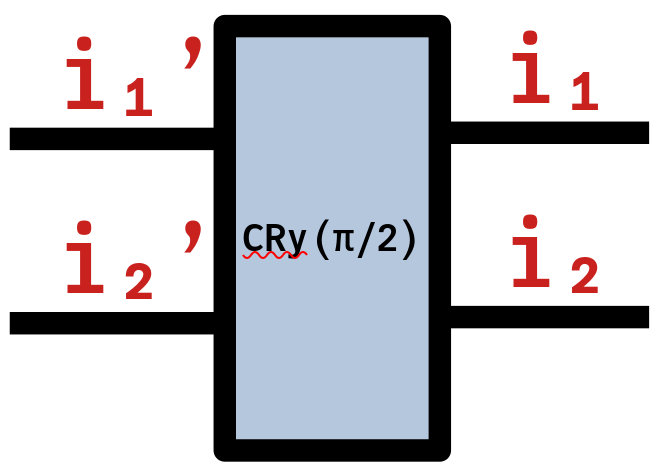
\includegraphics[width=0.5\textwidth]{
  slides/assets/CRy_pi_by_2.png
}
\end{center}
\vspace*{0.0cm}
\end{onlyenv}

%% \begin{onlyenv}<3->
%% ~\\
%% \end{onlyenv}

\begin{onlyenv}<3-3>
~\\
CRy($\pi$/2)|Z-Z+$\rangle$ =\\
\ \ \ \ |Z-X+$\rangle$ \\
~\\
\end{onlyenv}

\begin{onlyenv}<4->
\vspace*{0.0cm}
\begin{center}
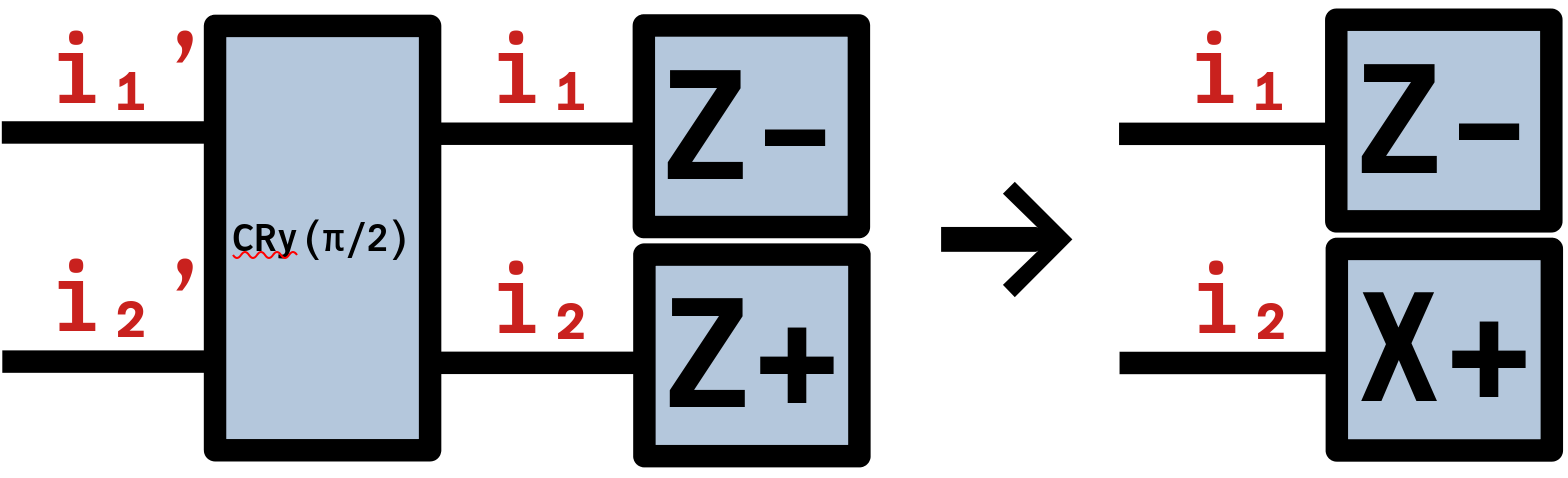
\includegraphics[width=1.0\textwidth]{
  slides/assets/CRyZm1Zp2_to_Zm1Xp2.png
}
\end{center}
\vspace*{0.0cm}
\end{onlyenv}

\end{column}

\end{columns}

\end{frame}
